\question State if the following statements are True or False, and justify. For all graphs, assume that edge weights are positive and distinct, unless otherwise stated.

\begin{parts}
  \part Adding some positive constant $k$ to every edge weight does not change the shortest path tree from vertex $S$.
  \begin{solution}[0.5in]
    False. 
    
    Consider the possible counterexample below.
    
    In this example, the original shortest path from A-C involves passing through B, but after adding a constant of 2, the shortest path is now directly taking the edge from A-C.
    
    Conceptually, when you add a constant to all your edges in your graph, longer paths will be disproportionately affected. 
  \end{solution}
  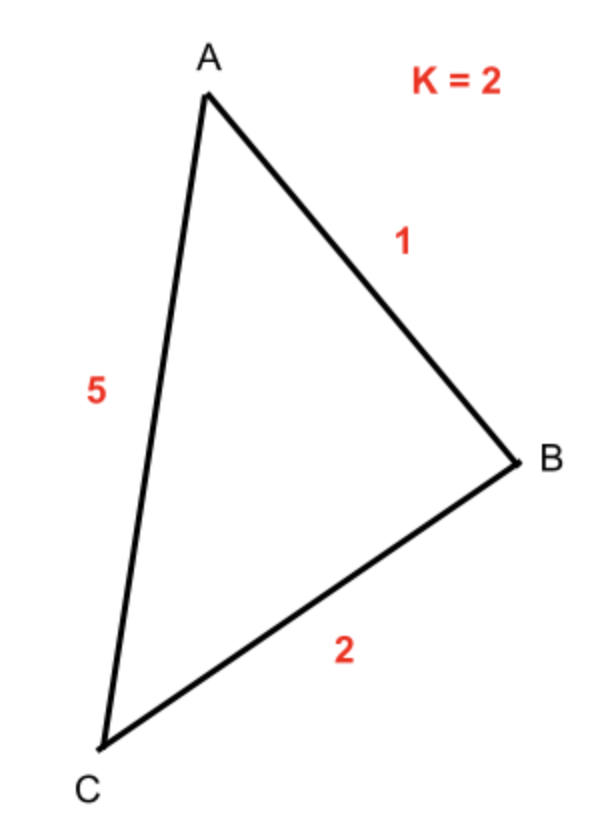
\includegraphics[scale=0.45]{topics/graphs/Graph_TF_Q3a.png}
  
  \part Doubling every edge weight does not change the shortest path tree.

  \begin{solution}[0.5in]
    True. 
    
     The explanation for this question should build off your reasoning for part a. By multiplying edge weights by a constant factor, all paths are still just an equal factor away from each other. We recommend referring to the previous counter example to show the correctness. 
  \end{solution}
  \part If the weight of each edge is decreased by 1, then the resulting shortest path in any graph from u to v is unchanged.
  \begin{solution}[0.5in]
    False. \\
    The effect of adding/subtracting a constant to/from each edge depends on the number of edges in a path. Subtracting 1 from every edge makes paths with more edges shorter. Subtracting from an edge can also make it negative.
  \end{solution}
  \part If a graph G has a unique MST, it must have unique edge weights.
  \begin{solution}[0.5in]
    False. \\
    The converse, however, is True: If a graph has unique edge weights, then the graph has a unique MST.
  \end{solution}
  \part Adding some positive constant $k$ to every edge weight does not change the minimum spanning tree.
  \begin{solution}[0.5in]
    True.
  \end{solution}
  \part Doubling every edge weight does not change the minimum spanning tree.
  \begin{solution}[0.5in]
    True. \\
    For the four parts above, we can consider when graph transformations affect the two algorithms:\\
    MST algorithms depend on the relative order of \emph{edge weights}. Hence, adding a constant, or doubling the edge weights does not alter the MST. (More broadly, any monotonically increasing function can be applied, such as squaring the edge weights, assuming they are all positive.) \\ \\
    Shortest path algorithms depend on the relative order of \emph{sums of edge weights}. More specifically, we are concerned about sums of edge weights that represent paths to vertices in the graphs. We can see then that adding a constant $k$ to all edge weights does alter the relative order of these sums. In fact, as $k$ increases, the algorithm becomes more biased towards paths that are shorter in \emph{hop-length}, i.e. number of vertices in the path. One intuitive way to think about this would be to make $k$ a very large number, tending towards infinity. Then all edge weights are approximately the same length, and shortest path algorithms will find the shortest path by hop-length, just like BFS. On the other hand, if we double every edge weight, the relative order of sums does not change. $2w_1 + 2w_2 + 2w_3 = 2(w_1 + w_2 + w_3)$. We see that we can factorize out the multiplier, and the ordering is still dependent on the original sums of edge weights. More broadly, we can consider any positive multiplication of edge weights to not affect shortest path trees.
  \end{solution}
  \part Let $(S, V-S)$ be a specific cut of the graph. If an edge $e$ is not the lightest edge across this cut, it cannot be a part of any MST.
  \begin{solution}[0.5in]
    False. 
    
    Consider the graph $\{(A, B, 1), (B, C, 2)\}$. Even though edge $(B, C)$ is not the lightest edge across the cut $\{A\}, \{B, C\}$, it is necessarily still a part of all MSTs (since this graph is a tree).
  \end{solution}
  \part If an edge $e$ is the lightest edge connected to vertex $S$, it must be a part of the shortest path tree from vertex $S$.
  \begin{solution}[0.5in]
    True. 
    
    If $e$ connects $S$ to $T$, then that must be the shortest path from $S$ to $T$. Assume there is some shorter path to $T$ from $S$. Then it must exit $S$ via edge $e'$ which has strictly larger weight than $e$, creating a contradiction.
  \end{solution}
  \part Consider a graph G, where every edge is nonnegative, except the edges adjacent to vertex s. Dijkstra’s usually fails on graphs with negative edge weights, however if we run Dijkstra’s starting from s, we will get the correct shortest paths tree.
  \begin{solution}[0.5in]
    True. \\
    Dijkstra’s fails if incorporating a negative edge not yet seen decreases the shortest path. In the case, all negative edges have been seen and added to the fringe. That means adding more edges to any forming path can only increase the total distance (since all other edge weights are nonnegative.
  \end{solution}
\end{parts}
